\documentclass[12pt]{article}
\usepackage{amsmath}
\usepackage{amssymb}
\usepackage{graphicx}
\usepackage{physics}
\usepackage{siunitx}
\usepackage{wrapfig}

\AtBeginDocument{\RenewCommandCopy\qty\SI}

\title{
    Chapter 18 End-of-Chapter Problems
    \\ \small
    Halliday \& Resnick, 10th Edition
}

\author{Doanld Aingworth IV}

\date{\small Hit me where it Matters}

\begin{document}
    \DeclareSIUnit{\cal}{\ cal}
    \DeclareSIUnit{\Cal}{\ Cal}
    \DeclareSIUnit{\calorie}{\ cal}
    \DeclareSIUnit{\Calorie}{\ Cal}
    \DeclareSIUnit{\fahrenheit}{^\circ F}

    \maketitle
    
    \pagebreak

    % \section{Question 4}
    %     \begin{wrapfigure}{r}{0.5\textwidth}
    %         \vspace{-30pt}
    %         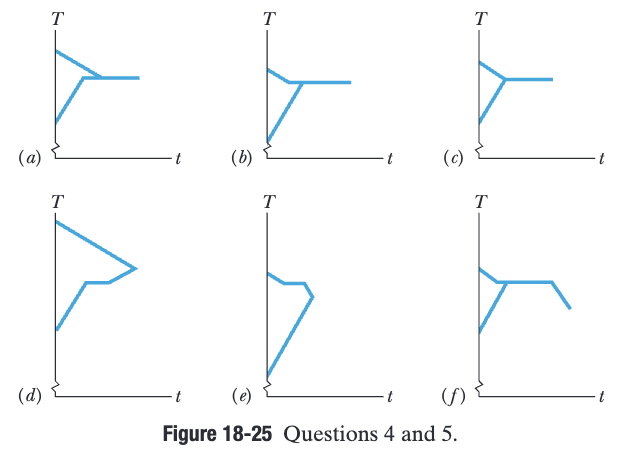
\includegraphics[width=0.5\textwidth]{picture_18-25.png} 
    %         % \label{fig:wrapfig}
    %     \end{wrapfigure}
    %     A sample A of liquid water and a sample B of ice, of identical mass, are placed in a thermally insulated container and allowed to come to thermal equilibrium. Figure 18-25$a$ is a sketch of the temperature T of the samples versus time t. (a) Is the equilibrium temperature above, below, or at the freezing point of water? (b) In reaching equilibrium, does the liquid partly freeze, fully freeze, or undergo no freezing? (c) Does the ice partly melt, fully melt, or undergo no melting?

    % \subsection{Solution}

    % \pagebreak
    % \section{Question 5}
    %     Question 4 continued: Graphs b through f of Fig. 18-25 are additional sketches of T versus t, of which one or more are impossible to produce. (a) Which is impossible and why? (b) In the possible ones, is the equilibrium temperature above, below, or at the freezing point of water? (c) As the possible situations reach equilibrium, does the liquid partly freeze, fully freeze, or undergo no freezing? Does the ice partly melt, fully melt, or undergo no melting?

    % \subsection{Solution}

    % \pagebreak
    \section{Problem 5}
        At what temperature is the Fahrenheit scale reading equal to (a) twice that of the Celsius scale and (b) half that of the Celsius scale?

        \subsection{Solution (a)}
            This is totally algebraic. 
            The formula from fahrenheit to celsius is $T_F = \frac{9}{5}T_C + 32^{\circ}$.
            To convert between the two, we need to set $T_F$ and $T_C$ to be equal.
            \begin{align}
                T_F &=  \frac{9}{5}T_F + 32^\circ\\
                \frac{4}{5}T_F  &=  -32^\circ\\
                T_F &=  \boxed{-40^\circ}
            \end{align}

        \subsection{Solution (b)}
            This is also algebraic.
            The Fahrenheit reading is half that of the Celsius scale reading.
            \begin{equation}
                T_F = \frac{1}{2}T_C \leftrightarrow 2 T_F = T_C
            \end{equation}

            We can substitute this into the conversion formula we used in part (a).
            \begin{align}
                T_F &=  \frac{9}{5}T_C + 32^\circ\\
                    &=  \frac{18}{5}T_F + 32^\circ\\
                \frac{13}{5}T_F &=  -32^\circ\\
                T_F &=  \boxed{-\frac{160}{13}^\circ \approx -12^\circ}
            \end{align}

            We can verify this.
            \begin{align}
                T_F &=  \frac{9}{5}T_C + 32^\circ\\
                T_C &=  \frac{5}{9}\left(T_F - 32^\circ\right)\\
                    &=  \frac{5}{9}\left(-\frac{160}{13}^\circ - 32^\circ\right)\\
                    &=  \frac{5}{9}\left(-\frac{576}{13}^\circ\right)\\
                    &=  -\frac{320}{13} = 2 * T_F\ \ \ \checkmark
            \end{align}


    \pagebreak
    \section{Problem 7}
        Suppose that on a linear temperature scale X, water boils at $-53.5$°X and freezes at $-170$°X. What is a temperature of 340 K on the X scale? (Approximate water's boiling point as 373 K.)

        \subsection{Solution}
            We can put together a fraction of differences here to get a ratio of Kelvin to X scale.
            I will be approximating water's freezing point at 273 K.
            \begin{gather}
                \frac{T_X}{T_K} =   \frac{-53.5 + 170}{373 - 273} = \frac{116.5}{100} = \frac{233}{200} = 1.165 \frac{^\circ X}{K}
            \end{gather}

            Now, we can test the difference in temperature between the freezing point and 340 K.
            \begin{gather}
                \Delta T    =   340 \unit{\kelvin} - 273 \unit{\kelvin} = 67 \unit{\kelvin}
            \end{gather}

            Multiplying this by the ratio of \textdegree X to Kelvin, we get the difference in X between the target temperature and the freezing point.
            \begin{gather}
                67 \unit{\kelvin} * \frac{233^\circ X}{200 \unit{\kelvin}} = \frac{15611}{200} ^\circ X = 78.055 ^\circ X
            \end{gather}

            Add this to the freezing point to get the target value.
            \begin{gather}
                -170 ^\circ X + 78.055 ^\circ X = \boxed{-91.945 ^\circ X}
            \end{gather}

    \pagebreak
    \section{Problem 9}
        A circular hole in an aluminum plate is 2.725 \unit{\centi\meter} in diameter at 0.000\unit{\celsius}. What is its diameter when the temperature of the plate is raised to 100.0\unit{\celsius}?

        \subsection{Solution}
            For any given linear dimension, the expansion is defined by a formula using the coefficient of linear expansion $\alpha$.
            \begin{equation}
                \Delta L = L\alpha \Delta T
            \end{equation}

            We are working with aluminium, so $\alpha = 23 \times 10^{-6}/\unit{\celsius}$. 
            Also given the temperature change of 100\unit{\celsius} and an initial diameter of $27.25 \times 10^{-3} \unit{\meter}$, we can calculate the change in diameter. 
            \begin{align}
                \Delta L    &=  (27.25 \times 10^{-3} \unit{\meter})(23 \times 10^{-6}/\unit{\celsius})(100 \unit{\celsius})\\
                    &=  6.2675 \times 10^{-5} \unit{\meter}
            \end{align}

            Adding $\Delta L$ to $L$, we get our final answer and length.
            \begin{align}
                L_f &=  L_i + \Delta L\\
                    &=  27.25 \times 10^{-3} \unit{\meter} + 6.2675 \times 10^{-5} \unit{\meter}\\
                    &=  \boxed{27.31 \times 10^{-3} \unit{\meter}}
            \end{align}

    \pagebreak
    \section{Problem 11}
        What is the volume of a lead ball at 30.00\unit{\celsius} if the ball's volume at 60.00\unit{\celsius} is 50.00 \unit{\centi\meter^3}?
        
        \subsection{Solution}
            This is a similar problem to Problem 9 (5). 
            The coefficient of volume expansion is equal to thrice the coefficient of linear expansion, the latter of which for lead is $29 \times 10^{-6}/\unit{\celsius}$.
            This leaves the coefficient of volume expansion as $\beta = 3 * 29 \times 10^{-6}/\unit{\celsius} = 87 \times 10^{-6}/\unit{\celsius}$.
            We can in turn use this to find the change in volume.
            \begin{align}
                \Delta V    &=  V_i \beta \Delta T\\
                    &=  (50 \unit{\centi\meter^3}) (87 \times 10^{-6}/\unit{\celsius}) (30 \unit{\celsius})\\
                    &=  130.5 \times 10^{-3} \unit{\centi\meter^3}
            \end{align}

            Add the change to the initial value to get the final value.
            \begin{align}
                V_f &=  V_i + \Delta V\\
                    &=  50.0 \unit{\centi\meter^3} + 130.5 \times 10^{-3} \unit{\centi\meter^3}\\
                    &=  50.1305 \unit{\centi\meter^3} \approx \boxed{50.13 \unit{\centi\meter^3}}
            \end{align}


    \pagebreak
    \section{Problem 15}
        A steel rod is 3.000 cm in diameter at 25.00°C. A brass ring has an interior diameter of 2.992 cm at 25.00°C. At what common temperature will the ring just slide onto the rod?

        \subsection{Solution}
        We can set up a couple formulas that must be equal to each other for this to hold. 
        $D_b$ will be the diameter of the brass ($\alpha_b = 19 \times 10^{-6}/\unit{\celsius}$) ring, while $D_s$ will be the diameter of the steel ($\alpha_s = 11 \times 10^{-6}/\unit{\celsius}$) rod. 
        \begin{gather}
            D_b + \Delta D_b = D_s + \Delta D_s\\
            D_b + D_b \alpha_b \Delta T = D_s + D_s \alpha_s \Delta T\\
            3 \unit{\centi\meter} + (3 \unit{\centi\meter}) (11 \times 10^{-6}/\unit{\celsius}) \Delta T = 2.992 \unit{\centi\meter} + (2.992 \unit{\centi\meter}) (19 \times 10^{-6}/\unit{\celsius}) \Delta T\\
            0.08 \times 10^{-3} \unit{\meter} + 0.33 \times 10^{-6} \unit{\meter/\celsius} * \Delta T = 0.56848 \times 10^{-6} \unit{\meter/\celsius} * \Delta T\\
            0.08 \times 10^{-3} \unit{\meter} = 0.23848 \times 10^{-6} \unit{\meter/\celsius} * \Delta T\\
            \Delta T = \frac{0.08 \times 10^{-3} \unit{\meter}}{0.23848 \times 10^{-6} \unit{\meter/\celsius}} = 335.458 \unit{\celsius}
        \end{gather}

        With this value of the change in the temperature, we can generate a total temperature.
        \begin{gather}
            T_f =   T_i + \Delta T  
                =   25.00 \unit{\celsius} + 335.458 \unit{\celsius}
                =   \boxed{360.458 \unit{\celsius}}
        \end{gather}
            

    \pagebreak
    \section{Problem 17}
        An aluminum cup of $100 \unit{\centi\meter^3}$ capacity is completely filled with glycerin at $22\unit{\celsius}$. How much glycerin, if any, will spill out of the cup if the temperature of both the cup and the glycerin is increased to $28\unit{\celsius}$? (The coefficient of volume expansion of glycerin is $5.1 \times 10^{-4}/\unit{\celsius}$.)

        \subsection{Solution}
            This is a non-experimental version, without calculus.
            Barring surface tension and assuming that there is no chance in hell that the cup will hold any more glycerin currently at its present temperature, the change in volume will be the volume that will spill.
            This can also give us the assumption that the initial volume of the cup and glycerin to be $100 \unit{\centi\meter^3}$. 
            We have a formula for this.
            \begin{align}
                \Delta T    &=  T_f - T_i
                    =   28\unit{\celsius} - 22 \unit{\celsius}
                    =   6 \unit{\celsius}\\
                \Delta V_g  &=  V_g \beta \Delta T\\
                    &=  (100\unit{\centi\meter^3}) (5.1 \times 10^{-4} /\unit{\celsius}) (6 \unit{\celsius})\\
                    &=  306 \times 10^{-3} \unit{\centi\meter^3}
            \end{align}

            We can also calculate the final volume of the aluminum ($\beta = 3\alpha = 69 \times 10^{-6}$).
            \begin{align}
                \Delta V_a  &=  V_a \beta \Delta T\\
                    &=  (100\unit{\centi\meter^3}) (69 \times 10^{-6} /\unit{\celsius}) (6 \unit{\celsius})\\
                    &=  41.4 \times 10^{-3} \unit{\centi\meter^3}
            \end{align}

            The difference between these would be the total volume that spills. 
            \begin{gather}
                306 \times 10^{-3} \unit{\centi\meter^3} - 41.4 \times 10^{-3} \unit{\centi\meter^3}    =   \boxed{264.6 \times 10^{-3} \unit{\centi\meter^3}}
            \end{gather}

    \pagebreak
    \section{Problem 21}
        \begin{wrapfigure}{r}{0.5\textwidth}
            \vspace{-30pt}
            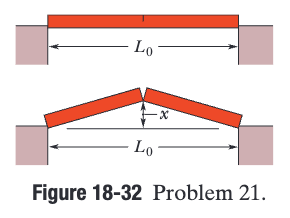
\includegraphics[width=0.5\textwidth]{picture_18-32.png} 
            % \label{fig:wrapfig}
        \end{wrapfigure}
        As a result of a temperature rise of 32 \unit{\celsius}, a bar with a crack at its center buckles upward (Fig. 18-32). The fixed distance $L_0$ is $3.77 \unit{\meter}$ and the coefficient of linear expansion of the bar is $25 \times 10^{-6}/\unit{\celsius}$. Find the rise x of the center.

        \subsection{Solution}
            We first find the final total length of the bar given the initial length.
            \begin{align}
                \Delta L &= L_0 \alpha \Delta T\\
                    &=  (3.77 \unit{\meter}) (25 \times 10^{-6}/\unit{\celsius}) (32 \unit{\celsius})\\
                    &=  3.016 \times 10^{-3} \unit{\meter}\\
                L_f &=  L_0 + \Delta L
                    =   3.77 \unit{\meter} + 3.016 \times 10^{-3} \unit{\meter}\\
                    &=  3.773016 \unit{\meter}
            \end{align}

            From this, we can use the Pythagoream Theorem to find the distance raised, bearing in mind that the values we use will be only half the magnitude of the values we found or know.
            \begin{align}
                x   &=  \sqrt{\left(\frac{3.773016}{2}\right)^2 - \left(\frac{3.77}{2}\right)^2}\\
                    &=  \sqrt{1.886508^2 - 1.885^2}\\
                    &=  \sqrt{5.69 \times 10^{-3} \unit{\meter^2}}
                    =   \boxed{0.0754 \unit{\meter}}
            \end{align}

    \pagebreak
    \section{Problem 23}
        A small electric immersion heater is used to heat 100 g of water for a cup of instant coffee. 
        The heater is labeled “200 watts” (it converts electrical energy to thermal energy at this rate). 
        Calculate the time required to bring all this water from 23.0\unit{\celsius} to 100\unit{\celsius}, ignoring any heat losses.

        \subsection{Solution}
            We have a formula for the heat transfered from the temperature.
            \begin{align}
                Q   &=  cm \Delta T
            \end{align}

            This has thermal energy in units of joules (\unit{\joule}).
            We can divide both by time to get the power (in units of watts (\unit{\joule/\second})) on the left side.
            \begin{align}
                \frac{Q}{t} &=  \frac{cm \Delta T}{t}\\
                P   &=  \frac{cm \Delta T}{t}
            \end{align}

            We can solve for the time.
            Recall the known mass and change in temperature, as well as the specific heat of water in \unit{\frac{\joule}{\kilo\gram\cdot\kelvin}}.
            \begin{align}
                t   &=  \frac{cm \Delta T}{P}\\
                    &=  \frac{\left( 4187\unit{\frac{\joule}{\kilo\gram\cdot\kelvin}} \right) \left( 0.1 \unit{\kilo\gram} \right) \left( 77 \unit{\kelvin} \right)}{200 \unit{\watt}}\\
                    &=  \frac{32239.9 \unit{\joule}}{200 \unit{\watt}}
                    =   \boxed{161.1995 \unit{\second} \approx 162 \unit{\second}}
            \end{align}

            Slight differences can be chocked up to sigfigs. 

    \pagebreak
    \section{Problem 25}
        A certain diet doctor encourages people to diet by drinking ice water. 
        His theory is that the body must burn off enough fat to raise the temperature of the water from 0.00°C to the body temperature of 37.0°C. 
        How many liters of ice water would have to be consumed to burn off 454 g (about 1 lb) of fat, assuming that burning this much fat requires 3500 Cal be transferred to the ice water? 
        Why is it not advisable to follow this diet? (One liter = $10^3 \unit{\centi\meter^3}$. 
        The density of water is $1.00 \unit{g/\centi\meter^3}$.)

        \subsection{Solution}
            We have a formula for this. 
            \begin{align}
                Q   &=  cm \Delta T
            \end{align}

            If we can find the mass of water required, we can find the volume given our known unit conversions, so we can isolate for that.
            \begin{gather}
                m   =   \frac{Q}{c \Delta T}
            \end{gather}

            The specific heat in this instance will be the specific heat of water ($c = 1 \unit{\frac{\calorie}{\gram\cdot\kelvin}} = 10^{-3} \unit{\frac{\Calorie}{\gram\cdot\kelvin}}$). 
            The change in temperature is 37.0\unit{\celsius}, which has identical magntude in Kelvin (\unit{K}). 
            \begin{align}
                m   &=  \frac{Q}{c \Delta T}
                    =   \frac{3500\unit{\Calorie}}{\left( 10^{-3} \unit{\frac{\Calorie}{\gram\cdot\kelvin}} \right) \left( 37.0 \unit{\kelvin} \right)}\\
                    &=  94594.6 \unit{\gram} * 1 \unit{\frac{\centi\meter^3}{\gram}} * 10^{-3} \unit{\frac{\liter}{\centi\meter^3}}\\
                    &=  \boxed{94.6 \unit{\liter}}
            \end{align}

            This requires drinking a \textit{lot} of ice water, about 47 and a half bottles of ice water per day. 
            I would not recommend it because it would take so long and would be so inefficient. 

    \pagebreak
    \section{Problem 27}
        Calculate the minimum amount of energy, in joules, required to completely melt 130 g of silver initially at 15.0\unit{\celsius}.

        \subsection{Solution}
        The amount of energy required for $130 \unit{\gram}$ of silver (melting point 1235 \unit{\kelvin}; $L_F = 105 \unit{\kilo\joule/\kilo\gram}$) can be separated into two parts: the energy necessary to heat it to melting temperature and the energy necessary to melt it at said temperature.
        \begin{align}
            E_\Sigma    &=  Q_{heat} + Q_{melt}
                =   cm\Delta T + Lm
        \end{align}

        Given these equations, we can calculate the total energy required.
        The specific heat of elemental solid silver is $236 \unit{\frac{\joule}{\kilo\gram\cdot\kelvin}}$.
        \begin{align}
            \Delta T    &=  1235 \unit{\kelvin} - 15.0 \unit{\celsius}
                =   1235 \unit{\kelvin} - 288.15 \unit{\kelvin}
                =   946.85 \unit{\kelvin}\\
            E_\Sigma    &=  \left( 236 \unit{\frac{\joule}{\kilo\gram\cdot\kelvin}} \right) (0.130 \unit{\kilo\gram}) (946.85 \unit{\kelvin}) + \left( 105 \unit{\frac{\joule}{\gram}} \right) \left( 130 \unit{\gram} \right)\\
                &=  29049.358 \unit{\joule} + 13650 \unit{joule}
                =   \boxed{42699.358 \unit{\joule} \approx 42700 \unit{\joule}}
        \end{align}

    \pagebreak
    \section{Problem 31}
        What mass of steam at 100\unit{\celsius} must be mixed with 150\unit{\gram} of ice at its melting point, in a thermally insulated container, to produce liquid water at 50\unit{\celsius}?

        \subsection{Solution}
        We can first calculate the amount of energy necessary for the ice to melt and heat to 50\unit{\celsius}. 
        \begin{align}
            Q   &=  cm \Delta T + Lm\\
                &=  \left( 4187 \unit{\frac{\joule}{\kilo\gram\cdot\kelvin}} \right) (0.15 \unit{\kilo\gram}) (50 \unit{\kelvin}) + (333 \unit{\joule/\gram}) (150 \unit{\gram})\\
                &=  31402.5 \unit{\joule} + 49950 \unit{\joule}
                =   81352.5 \unit{\joule}
        \end{align}

        This would be equal to the required energy from the steam to turn into liquid water at 50\unit{\celsius}.
        We can set up the same formula as above for the steam.
        \begin{gather}
            81352.5 \unit{\joule}   =   cm\Delta T + Lm = m(c\Delta T + L)\\
            \begin{align}
                m   &=  \frac{81352.5 \unit{\joule}}{c\Delta T + L}
                    =   \frac{81352.5 \unit{\joule}}{\left( 4187 \unit{\frac{\joule}{\kilo\gram\cdot\kelvin}} \right)(50\unit{\kelvin}) + 2256 \times 10^{3} \unit{\frac{\joule}{\kilo\gram}} }\\
                    &=  \frac{81352.5 \unit{\joule}}{ 209350 \unit{\frac{\joule}{\kilo\gram}} + 2256 \times 10^{3} \unit{\frac{\joule}{\kilo\gram}} }\\
                    &=  \frac{81352.5}{2465350} \unit{\kilo\gram}
            \end{align}\\
            m   =   \boxed{0.033 \unit{\kilo\gram} = 33 \unit{\gram}}
        \end{gather}

    \pagebreak
    \section{Problem 37}
        A person makes a quantity of iced tea by mixing 500\unit{\gram} of hot tea (essentially water) with an equal mass of ice at its melting point. 
        Assume the mixture has negligible energy exchanges with its environment. 
        If the tea's initial temperature is $T_i = 90\unit{\celsius}$, when thermal equilibrium is reached what are (a) the mixture's temperature $T_f$ and (b) the remaining mass $m_f$ of ice? If $T_i$ = 70°C, when thermal equilibrium is reached what are (c) $T_f$ and (d) $m_f$?

        \subsection{Solution (a)}
            First, we can calculate the energy that the tea have to would release to reduce its temperature to 0\unit{\celsius}, at which point it would start freezing if it released any more energy. 
            \begin{align}
                \Delta T    &=  0 \unit{\celsius} - 90 \unit{\celsius} = -90 \unit{\celsius}\\
                Q   &=  cm\Delta T\\
                    &=  \left( 4187 \unit{\frac{\joule}{\kilo\gram\cdot\kelvin}} \right) (0.5 \unit{\kilo\gram}) (-90 \unit{\celsius})\\
                    &=  -188415 \unit{\joule}
            \end{align}

            Next, we can calculate the amount of energy that would be absorbed by the ice completely melting.
            \begin{align}
                Q   &=  m L_F
                    =   \left( 333 \times 10^3 \unit{\joule/\kilo\gram} \right) \left( 0.5 \unit{\kilo\gram} \right)\\
                    &=  166500 \unit{\joule}
            \end{align}

            The magnitude of released energy is greater than the magnitude of absorbed energy, so all the ice will melt.
            To achieve thermal equilibrium, the energy absorbed by the ice would have to be equal to the energy released by the tea.
            We can find this by taking the average of the two quantities of energy found.
            From that, we can find the change in temperature of the water until it reaches thermal equilibrium.
            \begin{align}
                \frac{188415 + 166500}{2}   &=  177457.5\unit{\joule}   =   Q\\
                \Delta T    &=  \frac{Q}{cm}
                    =   \frac{-177457.5\unit{\joule}}{\left( 4187 \unit{\frac{\joule}{\kilo\gram\cdot\kelvin}} \right) (0.5 \unit{\kilo\gram})}
                    =   -84.766 \unit{\celsius}
            \end{align}

            This we can add to the initial temperature to find the final temperature.
            \begin{gather}
                T_f = T_i + \Delta T = 90 \unit{\celsius} - 84.766 \unit{\celsius} = \boxed{5.2 \unit{\celsius}}
            \end{gather}

        \subsection{Solution (b)}
            As established, all the ice melts, so $m_f = \boxed{0\unit{\gram}}$. 

        \subsection{Solution (c)}
            The ice would take the same amount of energy to melt, so $Q_{ice} = 166500 \unit{\joule}$.
            Knowing this, we should calculate the amount of energy to reduce all the tea to $0\unit{\celsius}$. 
            \begin{align}
                \Delta T    &=  0 \unit{\celsius} - 70 \unit{\celsius} = -70 \unit{\celsius}\\
                Q   &=  cm\Delta T\\
                    &=  \left( 4187 \unit{\frac{\joule}{\kilo\gram\cdot\kelvin}} \right) (0.5 \unit{\kilo\gram}) (-70 \unit{\celsius})\\
                    &=  -146545 \unit{\joule}
            \end{align}

            The magnitude of absorbed energy is greater than the magnitude of released energy, so less than all the ice will melt but all the water will reach \boxed{0\unit{\celsius}}.

        \subsection{Solution (d)}
            To achieve thermal equilibrium, the energy absorbed by the ice would have to be equal to the energy released by the tea.
            We can find this by taking the average of the two quantities of energy found.
            From that, we can find the lost mass of the ice when it reaches thermal equilibrium.
            \begin{align}
                \frac{146545 + 166500}{2}   &=  156522.5\unit{\joule}   =   Q\\
                Q   &=  m L_F\\
                m   &=  \frac{Q}{L_F}
                    =   \frac{156522.5\unit{\joule}}{333 \times 10^3 \unit{\joule/\kilo\gram}}\\
                    &=  0.47 \unit{\kilo\gram}
            \end{align}

            Subtract this from the total mass of the ice to find the final mass of ice not melted.
            \begin{equation}
                m_f =   0.5 \unit{\kilo\gram} - 0.47 \unit{\kilo\gram}  =   \boxed{0.03 \unit{\kilo\gram}}
            \end{equation}

        \subsection{Differential Equations Remark}
            This could be done with some differential equations.
            Presumably, the ice that is unfrozen would automatically start warming up and the full energy transfer would not be instantaneous, so we could set up a time variable and set up a function of the mass over time. 
            \begin{gather}
                Q   =   mL_F\\
                \dv{Q}{t} = \dv{m}{t} L_F
            \end{gather}


    \pagebreak
    \section{Problem 41}
        (a) Two 50 g ice cubes are dropped into 200\unit{\gram} of water in a thermally insulated container. 
        If the water is initially at 25\unit{\celsius}, and the ice comes directly from a freezer at -15\unit{\celsius}, what is the final temperature at thermal equilibrium? 
        (b) What is the final temperature if only one ice cube is used?
    
        \subsection{Solution (a)}
            First find the total necessary energy for the ice to warm all the way up to $25\unit{\celsius}$ water and the water to cold all the way down to $-15\unit{\celsius}$.
            First the heating of the ice.
            { \small
            \begin{align}
                Q_{\Sigma i}    &=  c_i m_i \Delta T_i + L_F m_i + c_w m_i \Delta T_w\\
                    &=  (0.1 \unit{\kilo\gram}) \left( \left( 2220 \unit{\frac{\joule}{\kilo\gram\cdot\kelvin}} \right) \left( 15 \unit{\kelvin} \right) + 333 \times 10^3 \unit{\frac{\joule}{\kilo\gram}} + \left( 4187 \unit{\frac{\joule}{\kilo\gram\cdot\kelvin}} \right) \left( 25 \unit{\kelvin} \right) \right)\\
                    &=  \left( 0.1 \unit{\kilo\gram} \right) \left( 33300 \unit{\frac{\joule}{\kilo\gram}} + 333000 \unit{\frac{\joule}{\kilo\gram}} + 104675 \unit{\frac{\joule}{\kilo\gram}} \right)\\
                    &=  (0.1 \unit{\kilo\gram}) \left( 470975 \unit{\frac{\joule}{\kilo\gram}} \right)
                    =   47097.5 \unit{\joule}
            \end{align}}

            Then, the cooling of the water.
            \begin{align}
                Q_{\Sigma w}    &=  c_i m_w \Delta T_i + L_F m_w + c_w m_w \Delta T_w\\
                    &=  (0.2 \unit{\kilo\gram}) \left( 470975 \unit{\frac{\joule}{\kilo\gram}} \right)
                    =   94195 \unit{\joule}
            \end{align}

            Take the average of these two to find the total energy used. 
            \begin{gather}
                \frac{47097.5 \unit{\joule} + 94195 \unit{\joule}}{2}   =   70646.25 \unit{\joule}
            \end{gather}

            The last thing we can do is go through the processes until there is no energy left, going from the baseline of the 200\unit{\gram} of water.
            We start with the cooling to 0\unit{\celsius}. 
            \begin{align}
                70646.25 \unit{\joule} - c_w m_i \Delta T_w
                    &=  70646.25 \unit{\joule} - \left( 4187 \unit{\frac{\joule}{\kilo\gram\cdot\kelvin}} \right) (0.2 \unit{\kilo\gram}) \left( 25 \unit{\kelvin} \right)\\
                    &=  70646.25 \unit{\joule} - 20935 \unit{\joule}
                    =   49711.25 \unit{\joule}
            \end{align}

            Next is the freezing.
            \begin{align}
                49711.25 \unit{\joule} - m_w L_F
                    &=  49711.25 \unit{\joule} - (0.2 \unit{\kilo\gram}) \left( 333000 \unit{\frac{\joule}{\kilo\gram}} \right)\\
                    &=  49711.25 \unit{\joule} - 66600 \unit{\joule}
                    =   -16888.75 \unit{\joule}
            \end{align}

            Since this is new negative, the alotted energy has run out and thermal equlbrium has been reached at \boxed{0\unit{\celsius}}. 

        \subsection{Solution (b)}
        Take the energy to freeze all the water.
        \begin{align}
            Q_w &=  cm \Delta T
                =   4187 * 0.2 * 25
                =   20935 \unit{\joule}
        \end{align}
        
        Then, take the energy to melt all the ice.
        \begin{align}
            Q_i &=  cm \Delta T + m L_F
                =   2220 * 0.05 * 15 + 333000 * 0.05\\
                &=  1665 + 16650
                =   18315 \unit{\joule}
        \end{align}

        Average these two. 
        \begin{align}
            \frac{20935 \unit{\joule} + 18315 \unit{\joule}}{2} = 19625 \unit{\joule}
        \end{align}

        Apply that and find the value of $\Delta T$ for the water after removing the energy ncessary to warm and melt the ice, then from that, find $T_f$ of the water. 
        \begin{align}
            Q   &=  cm \Delta T\\
            \Delta T    &=  \frac{Q}{cm}
                =   \frac{18315}{4187 * 0.2}
                =   \frac{18315}{837.4}
                =   21.87 \unit{\kelvin}\\
            T_f &=  25 \unit{\celsius} - 21.87 \unit{\kelvin}
                =   3.13 \unit{\kelvin}
        \end{align}

        Now we use our known quantities to find the final $T_f$.
        \begin{align}
            0   &=  (cm \Delta T)_1 + (cm \Delta T)_2\\
                &=  4187 \left( 0.05 (T_f - 0) + 0.2 (T_f - 3.13) \right)\\
                &=  4187 \left( 0.25 T_f - 0.2 * 3.13 \right)\\
            0   &=  0.25 T_f - 0.2 * 3.13
                =   T_f - 0.8 * 3.13\\
            T_f &=  0.8 * 3.13
                =   \boxed{2.5 \unit{\celsius}}
        \end{align}
        

    \pagebreak
    \section{Problem 43}
        \begin{wrapfigure}{r}{0.25\textwidth}
            \vspace{-30pt}
            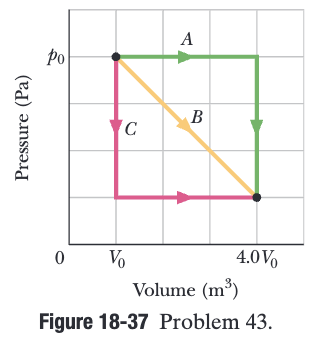
\includegraphics[width=0.25\textwidth]{picture_18-37.png} 
            % \label{fig:wrapfig}
        \end{wrapfigure}
        In Fig. 18-37, a gas sample expands from $V_0$ to $4.0 V_0$ while its pressure decreases from $p_0$ to $p_0/4.0$. 
        If $V_0 = 1.0 \unit{\meter^3}$ and $p_0 = 40 \unit{\pascal}$, how much work is done by the gas if its pressure changes with volume via (a) path A, (b) path B, and (c) path C?

        \subsection{Solution (a)}
            We have a formula for the work done by a gas from its pressure and volume.
            \begin{equation}
                W = \int\, dW = \int_{V_i}^{V_f} p \,dV 
            \end{equation}

            Following from this, we can create a formula for the pressure from the volume.
            \begin{equation}
                p(V) = \begin{cases}
                    p_0     &\text{if } V_0 < V < 4 V_0\\
                    p_0/4   &\text{if } V = 4 V_0
                \end{cases}
            \end{equation}

            Knowing this, we can develop the integral above and solve it.
            \begin{align}
                W   &=  \int_{V_i}^{V_f} p(V) \,dV 
                    =   \int_{V_0}^{4V_0} p_0 \,dV
                    =   \left[ p_0*V \right]_{V_0}^{4V_0}\\
                    &=  4 V_0 p_0 - V_0 p_0
                    =   3 V_0 p_0
                    =   3 * 1 \unit{\meter^3} * 40 \unit{\pascal}\\
                    &=  \boxed{120 \unit{\joule}}
            \end{align}

        \subsection{Solution (b)}
            Here is the formula for the pressure from the volume.
            \begin{equation}
                p(V)    = \frac{p_f - p_i}{V_f - V_i}V + b    = \frac{10 - 40}{4 - 1} V + 50  = -\frac{30}{3} V + 50  = 50 - 10V 
            \end{equation}

            We next apply that to the integral from part (a) and perform the integral.
            \begin{align}
                W   &=  \int_{V_i}^{V_f} p(V) \,dV 
                    =   \int_{V_0}^{4V_0} 50 - 10V \,dV
                    =   \left[ 50V - 5 V^2 \right]_{V_0}^{4V_0}\\
                    &=  \left( 50 * 4V_0 - 5*(4 V_0)^2 \right) - \left( 50 V_0 - 5 (V_0)^2 \right)\\
                    &=  200 V_0 - 80 V_0^2 - 50 V_0 + 5 V_0^2
                    =   150 V_0 - 75 V_0^2\\
                    &=  150 - 75 \unit{\joule}
                    =   \boxed{75 \unit{\joule}}
            \end{align}

        \subsection{Solution (c)}
            Here is the new formula for the pressure from the volume.
            \begin{equation}
                p(V) = \begin{cases}
                    p_0/4   &\text{if } V_0 < V < 4 V_0\\
                    p_0.    &\text{if } V = 4 V_0
                \end{cases}
            \end{equation}

            Then, we apply the integral. 
            \begin{align}
                W   &=  \int_{V_i}^{V_f} p(V) \,dV 
                    =   \int_{V_0}^{4V_0} \frac{p_0}{4} \,dV
                    =   \left[ \frac{p_0}{4}*V \right]_{V_0}^{4V_0}\\
                    &=  \frac{4}{4} V_0 p_0 - \frac{1}{4} V_0 p_0
                    =   \frac{3}{4} V_0 p_0
                    =   \frac{3}{4} * 1 \unit{\meter^3} * 40 \unit{\pascal}\\
                    &=  \boxed{30 \unit{\joule}}
            \end{align}
        

    \pagebreak
    \section{Problem 45}
        \begin{wrapfigure}{r}{0.25\textwidth}
            \vspace{-30pt}
            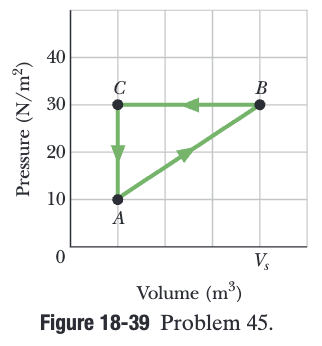
\includegraphics[width=0.25\textwidth]{picture_18-39.png} 
            % \label{fig:wrapfig}
        \end{wrapfigure}
        A gas within a closed chamber undergoes the cycle shown in the $p-V$ diagram of Fig. 18-39. 
        The horizontal scale is set by $V_s = 4.0 \unit{\meter^3}$. 
        Calculate the net energy added to the system as heat during one complete cycle.

        \subsection{Solution}
        We can set up a triad of integrals for the three parts of this path.
        Before that, we can put together a formula for $p(V)$ from A to B.
        \begin{gather}
            p(V)    =   \frac{\Delta p}{\Delta V}V + b  =   \frac{30 - 10}{V_s - \frac{1}{4}V_s}V + b   =   \frac{20}{4 - 1}V + b   =   \frac{20}{3}V + b\\
            b   =   p(1) - \frac{20}{3} * 1 =   10 - \frac{20}{3}   =   \frac{10}{3}\\
            W_{AB}  =   \int_{\frac{V_s}{4}}^{V_s} p_{AB}(V) \,dV   =   \int_{1\unit{\meter^3}}^{4\unit{\meter^3}} \frac{20}{3}V + \frac{10}{3} \,dV\\
            W_{BC}  =   \int_{V_s}^{\frac{V_s}{4}} p_{BC}(V) \,dV   =   \int_{4\unit{\meter^3}}^{1\unit{\meter^3}} 30 \,dV\\
            W_{CA}  =   \int_{V_s/4}^{V_s/4} p_{CA}(V) \,dV =   0
        \end{gather}

        That last one is automatically set to zero because the start and end points are equal.
        We can find the answer by adding these three together.
        \begin{align}
            W_{ABC} &=  W_{AB} + W_{BC} + W_{CA}\\
                &=  \int_{1\unit{\meter^3}}^{4\unit{\meter^3}} \frac{20}{3}V + \frac{10}{3} \,dV + \int_{4\unit{\meter^3}}^{1\unit{\meter^3}} 30 \,dV + 0\\
                &=  \left[ \frac{10}{3}V^2 + \frac{10}{3}V \right]_{1\unit{\meter^3}}^{4\unit{\meter^3}} + \left[ 30V \right]_{4\unit{\meter^3}}^{1\unit{\meter^3}}\\
                &=  \frac{10}{3}(16 - 1) + \frac{10}{3}(4 - 1) + 30(1 - 4)\\
                &=  50 \unit{\joule} + 10 \unit{\joule} - 90 \unit{\joule}
                =   -30 \unit{\joule}
        \end{align}

        As such, a total of \boxed{-30 \unit{\joule}} of energy is added as heat during one cycle.

    \pagebreak
    \section{Problem 47}
        \begin{wrapfigure}{r}{0.25\textwidth}
            \vspace{-30pt}
            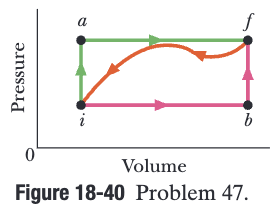
\includegraphics[width=0.25\textwidth]{picture_18-40.png} 
            % \label{fig:wrapfig}
        \end{wrapfigure}
        When a system is taken from state $i$ to state $f$ along path $iaf$ in Fig. 18-40, $Q = 50 \unit{\calorie}$ and $W = 20 \unit{\calorie}$. 
        Along path $ibf$, $Q = 36 \unit{\calorie}$. 
        (a) What is $W$ along path $ibf$? 
        (b) If $W = -13 \unit{\calorie}$ for the return path $fi$, what is $Q$ for this path? 
        (c) If $E_{int,i} = 10 \unit{\calorie}$, what is $E_{int,f}$? 
        If $E_{int,b} = 22 \unit{\calorie}$, what is $Q$ for (d) path $ib$ and (e) path $bf$?

        \subsection{Solution (a)}
            While $Q$ and $W$ are path dependant, $\Delta E_{int}$ is not.
            Since $\Delta E_{int} = Q - W$, we can write and solve an equation for both $iaf$ and $ibf$. 
            \begin{gather}
                Q_{iaf} - W_{iaf} = Q_{iaf} - W_{ibf}\\
                50 \unit{\calorie} - 20 \unit{\calorie} = 36 \unit{\calorie} - W_{ibf}\\
                W_{ibf} = 36 \unit{\calorie} - 30 \unit{\calorie} = \boxed{6 \unit{\calorie}}
            \end{gather}

        \subsection{Solution (b)}
            The answer can be found similarly, bearing in mind that since the start and end points are opposite, $\Delta E_{iaf} = -\Delta E_{fi}$. 
            We can give a formula.
            \begin{gather}
                \Delta E_{iaf} = -\Delta E_{fi}\\
                Q{iaf} - W_{iaf} = 30 \unit{\cal} = W_{fi} - Q_{fi} = -13\unit{\calorie} - Q_{fi}\\
                Q_{fi} = -13 \unit{\calorie} - 30 \unit{\calorie} = \boxed{-43 \unit{\calorie}}
            \end{gather}

        \subsection{Solution (c)}
            Add the change in energy to the initial energy to get the final energy.
            \begin{align}
                E_{int,f}   &=  E_{int,i} + \Delta E_{int}
                    =   10 \unit{\calorie} + 30 \unit{\calorie}
                    =   \boxed{40 \unit{\calorie}}
            \end{align}

        \subsection{Solution (d)}
            I assume that the value of $E_{int,i}$ remains the same.
            Since the volume changes but the pressure does not, $W \neq 0$. 
            However, the volume does not change along the path of $bf$, so $W_{ib} = W_{ibf} = 6 \unit{\calorie}$. 
            We also have an equation of path independence of change in energy, so we can use that. 
            \begin{gather}
                \Delta E_{int} = E_{int,b} - E_{int,i} = Q_{ib} - W_{ib}\\
                Q_{ib} = E_{int,b} - E_{int,i} + W_{ib} = 22 - 10 + 6 = \boxed{18 \unit{\calorie}}
            \end{gather}

        \subsection{Solution (e)}
            We know that $W = 0$ and $E_{int,f} = 40 \unit{\calorie}$.
            As such, we can find $\Delta E_{int,bf}$ and from that $Q$.
            \begin{gather}
                \Delta E_{int,bf} = E_{int,f} - E_{int,b} = 40 - 22 = 18 \unit{\calorie}\\
                \Delta E_{int,bf} = Q - W = Q - 0 = Q = \boxed{18 \unit{\calorie}}
            \end{gather}


    \pagebreak
    \section{Problem 49}
        \begin{wrapfigure}{r}{0.25\textwidth}
            \vspace{-30pt}
            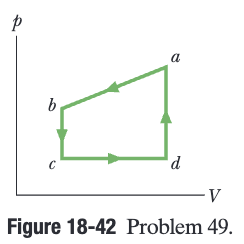
\includegraphics[width=0.25\textwidth]{picture_18-42.png} 
            % \label{fig:wrapfig}
        \end{wrapfigure}
        Figure 18-42 represents a closed cycle for a gas (the figure is not drawn to scale). 
        The change in the internal energy of the gas as it moves from $a$ to $c$ along the path $abc$ is $-200 \unit{\joule}$.
        As it moves from $c$ to $d$, $180 \unit{\joule}$ must be transferred to it as heat. 
        An additional transfer of $80 \unit{\joule}$ to it as heat is needed as it moves from $d$ to $a$. 
        How much work is done on the gas as it moves from $c$ to $d$?

        \subsection{Solution}
            This requires a system of equations.
            \begin{align}
                -200\unit{\joule}   &=  Q_{ab} - W_{ab} + Q_{bc} - W_{bc} = \Delta E_{int,ac} = -\Delta E_{int,ca}\\
                180 \unit{\joule}   &=  Q_{cd}\\
                80 \unit{\joule}    &=  Q_{da}
            \end{align}

            Along vertical pathways, $W = 0$, so we can apply that knowledge to this system of equations.
            We can also add the formula for $\Delta E_{int,cda}$. 
            \begin{align}
                -200\unit{\joule}   &=  Q_{ab} - W_{ab} + Q_{bc}\\
                180 \unit{\joule}   &=  Q_{cd}\\
                80 \unit{\joule}    &=  Q_{da} - W_{da} = \Delta E_{int,da}\\
                \Delta E_{int,cda}  &=  Q_{cd} - W_{cd} + Q_{da} - W_{da} = 200 \unit{\joule}
            \end{align}

            We can substitute known values into our last equation, including the fact that on vertical lines, $W = 0$.
            \begin{align}
                200 \unit{\joule}   &=  180 \unit{\joule} - W_{cd} + 80 \unit{\joule}\\
                W_{cd}  &=  180 \unit{\joule} + 80 \unit{\joule} - 200 \unit{\joule} = \boxed{60 \unit{\joule}}
            \end{align}

            This was a fun problem. 
            My compliments to the chef. 

    \pagebreak
    \section{Problem 51}
        A sphere of radius $0.500\unit{\meter}$, temperature $27.0\unit{\celsius}$, and emissivity 0.850 is located in an environment of temperature $77.0\unit{\celsius}$.
        At what rate does the sphere (a) emit and (b) absorb thermal radiation? 
        (c) What is the sphere's net rate of energy exchange?

        \subsection{Solution (a)}
            We have a formula for radiation emitted. 
            \begin{equation}
                P_{rad} =   \sigma \varepsilon A T^4
            \end{equation}

            Since A is the area of the sphere, we should first calculate that. 
            \begin{align}
                A   &=  4\pi r^2
                    =   4\pi 0.5^2
                    =   \pi \unit{\meter^2}
            \end{align}

            We can then convert the temperature from Celsius to Kelvin and use that to find the answer.
            \begin{align}
                T_{\unit{\kelvin}}  &=  T_{\unit{\celsius}} + 273.15 \unit{\degree}
                    =   27.0 \unit{\celsius} + 273.15 \unit{\degree}
                    =   300.15\unit{\kelvin}\\
                P_{rad} &=  (5.6704 \times 10^{-8} \unit{\watt/\meter^2\cdot\kelvin^4}) (0.850) (\pi \unit{\meter^2}) (300.15 \unit{\kelvin})^4\\
                    &=  \boxed{1228.868 \unit{\watt}}
            \end{align}

        \subsection{Solution (b)}
            We have a formula for environmental radiation absorbed.
            \begin{equation}
                P_{abs} =   \sigma \varepsilon A T_{env}^4
            \end{equation}

            The area of the sphere remains the same, so we can then convert the temperature from Celsius to Kelvin and use that to find the answer.
            \begin{align}
                T_{\unit{\kelvin}}  &=  T_{\unit{\celsius}} + 273.15 \unit{\degree}
                    =   77.0 \unit{\celsius} + 273.15 \unit{\degree}
                    =   350.15\unit{\kelvin}\\
                P_{abs} &=  (5.6704 \times 10^{-8} \unit{\watt/\meter^2\cdot\kelvin^4}) (0.850) (\pi \unit{\meter^2}) (350.15 \unit{\kelvin})^4\\
                    &=  \boxed{2275.980 \unit{\watt}}
            \end{align}

            These two equations seem to be practically the same, as if it is merely about a change in temperature abruptly over a specific area.

        \subsection{Solution (c)}
            The net radiation is the radiation emitted minus the radiation absorbed.
            \begin{equation}
                P_\Sigma    =   P_{rad} - P_{abs}
                    =   1228.868 \unit{\watt} - 2275.980 \unit{\watt}
                    =   -1047.112 \unit{\watt}
            \end{equation}

            This means that on net, it absorbs \boxed{1047.112 \unit{\watt}}. 


    \pagebreak
    \section{Problem 53}
        \begin{wrapfigure}{r}{0.25\textwidth}
            \vspace{-30pt}
            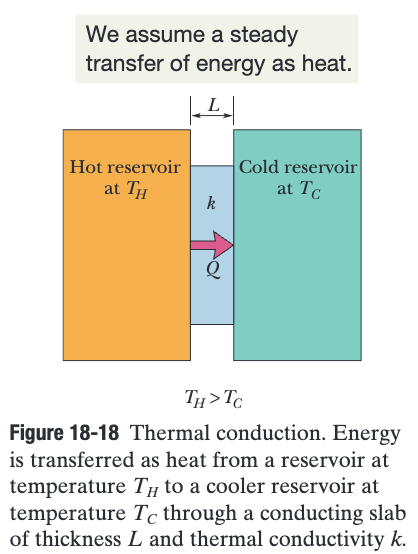
\includegraphics[width=0.25\textwidth]{picture_18-18.png} 
            % \label{fig:wrapfig}
        \end{wrapfigure}
        Consider the slab shown in Fig. 18-18. 
        Suppose that $L = 25.0 \unit{\centi\meter}$, $A = 90.0 \unit{\centi\meter^2}$, and the material is copper. 
        If $T_H = 125\unit{\celsius}$, $T_C = 10.0\unit{\celsius}$, and a steady state is reached, find the conduction rate through the slab.

        \subsection{Solution}
            The conduction rate is established in an equation.
            \begin{equation}
                P_{cond} = \frac{Q}{t} = kA \frac{T_H - T_C}{L}
            \end{equation}

            The second half of this would be the source of our interest.
            The thermal conductivity of copper is $401 \unit{\watt/\meter\cdot\kelvin}$.
            \begin{align}
                P_{cond}    &=  (401 \unit{\watt/\meter\cdot\kelvin}) (90 \times 10^{-4} \unit{\meter}) \frac{125 \unit{\celsius} - 10 \unit{\celsius}}{0.25 \unit{\meter}}\\
                    &=  (3.609 \unit{\watt\cdot\meter/\kelvin})\frac{115\unit{\kelvin}}{0.25\unit{\meter}}
                    =   \boxed{1660.14 \unit{\watt}}
            \end{align}
            


    \pagebreak
    \section{Problem 57}
        (a) What is the rate of energy loss in watts per square meter through a glass window 3.0 mm thick if the outside temperature is $-20\unit{\fahrenheit}$ and the inside temperature is +72°F? 
        (b) A storm window having the same thickness of glass is installed parallel to the first window, with an air gap of 7.5 cm between the two windows. 
        What now is the rate of energy loss if conduction is the only important energy-loss mechanism?

        \subsection{Solution (a)}
            We use the equation for the conductivity of a volume.
            % Suppose that the area A is 1 \unit{\meter^2}.
            The thermal conductivity of window glass is $1.0 \unit{\watt/\meter\cdot\kelvin}$. 
            Note that we should first convert $\Delta T$ from Fahrenheit/Rankine to Celsius/Kelvin.
            \begin{align}
                \Delta T_{\unit{\fahrenheit}}   &=  72 \unit{\fahrenheit} + 20 \unit{\fahrenheit}
                    =   92 \unit{\fahrenheit}\\
                \Delta T_{\unit{\kelvin}}  &=  \frac{9}{5} \Delta T_{\unit{\kelvin}}
                    =   \frac{5 \unit{\kelvin}}{9 \unit{\fahrenheit}} * 92 \unit{\fahrenheit}
                    =   \frac{460}{9} \unit{\kelvin}\\
                P_{cond}    &=  kA\frac{T_H - T_C}{L}\\
                \frac{P_{cond}}{A}  &=  k\frac{T_H - T_C}{L}
                    =   (1.0 \unit{\watt/\meter\cdot\kelvin}) \frac{460/9 \unit{\kelvin}}{3 \times 10^{-3} \unit{\meter}}\\
                    &=  \boxed{17.04 \times 10^3 \unit{\watt/\meter^2}}
            \end{align}

        \subsection{Solution (b)}
            There exists a previously established equation for the conduction of any number of materials, which we can use here.
            We can assume the air to be dry air, with a relatively low thermal conductivity 0.026 \unit{\watt/\meter\cdot\kelvin}.
            We also assume the two windows are of the same material.
            \begin{align}
                P_{cond}    &=  \frac{A\Delta T}{\sum(L/k)}\\
                \frac{P_{cond}}{A}  &=  \frac{\Delta T}{\sum(L/k)}
                    =   \frac{460/9 \unit{\kelvin}}{\frac{0.003}{1} + \frac{0.075}{0.026} + \frac{0.003}{1}}\\
                    &=  \frac{460/9}{0.003 + 2.8846 + 0.003}
                    =   \frac{460/9}{2.891}\\
                    &=  \boxed{17.7 \unit{\watt/\meter^2}}
            \end{align}

    \pagebreak
    \section{Problem 59}
        \begin{wrapfigure}{r}{0.25\textwidth}
            \vspace{-30pt}
            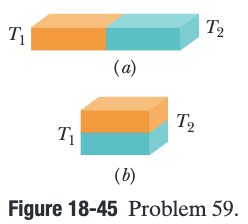
\includegraphics[width=0.25\textwidth]{picture_18-45.png} 
            % \label{fig:wrapfig}
        \end{wrapfigure}
        In Fig. 18-45$a$, two identical rectangular rods of metal are welded end to end, with a temperature of $T_1 = 0\unit{\celsius}$ on the left side and a temperature of $T_2 = 100\unit{\celsius}$ on the right side. 
        In 2.0 min, $10 \unit{\joule}$ is conducted at a constant rate from the right side to the left side.
        How much time would be required to conduct $10 \unit{\joule}$ if the rods were welded side to side as in Fig. 18-45$b$?

        \subsection{Solution}
            In this case, the change in temperature comes first.
            \begin{equation}
                \Delta T    =   T_2 - T_1
                    =   100 \unit{\celsius} - 0 \unit{\celsius}
                    =   100 \unit{\kelvin}
            \end{equation}

            We have a formula for the conduction, which relates to the energy conducted.
            \begin{gather}
                P_{cond;a}    =   \frac{Q}{t}
                    =   \frac{10 \unit{\joule}}{120 \unit{\second}}
                    =   kA\frac{\Delta T}{L}
            \end{gather}

            Case (b) has twice the surface area and half the length.
            \begin{gather}
                P_{cond;b}  =   \frac{10 \unit{\joule}}{t}
                    =   k*2A\frac{\Delta T}{L/2}
            \end{gather}

            We can isolate the values shared values, then apply the tramsistive property.
            \begin{gather}
                \frac{1}{120 \unit{\second}}    =   kA\frac{\Delta T}{L * 10 \unit{\joule}}\\
                \frac{1}{4t}    =   kA\frac{\Delta T}{L * 10 \unit{\joule}}\\
                \frac{1}{4t}    =   \frac{1}{120 \unit{\second}}\\
                t   =   \boxed{30 \unit{\second}}
            \end{gather}


    \pagebreak
    \section{Problem 63}
        \begin{wrapfigure}{r}{0.5\textwidth}
            \vspace{-30pt}
            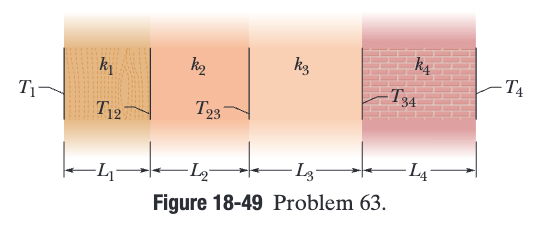
\includegraphics[width=0.5\textwidth]{picture_18-49.png} 
            % \label{fig:wrapfig}
        \end{wrapfigure}
        Figure 18-49 shows (in cross section) a wall consisting of four layers, with thermal conductivities $k_1 = 0.060 \unit{\watt/\meter\cdot\kelvin}$, $k_3 = 0.040 \unit{\watt/\meter\cdot\kelvin}$, and $k_4 = 0.12 \unit{\watt/\meter\cdot\kelvin}$ ($k_2$ is not known). 
        The layer thicknesses are $L_1 = 1.5 \unit{\centi\meter}$, $L_3 = 2.8 \unit{\centi\meter}$, and $L_4 = 3.5 \unit{\centi\meter}$ ($L_2$ is not known). 
        The known temperatures are $T_1 = 30 \unit{\celsius}$, $T_{12} = 25 \unit{\celsius}$, and $T_4 = -10\unit{\celsius}$. 
        Energy transfer through the wall is steady. 
        What is interface temperature $T_{34}$?

        \subsection{Solution}
            We have some formulas usable for this.
            First among these would be the formula for the conductivity. 
            \begin{equation}
                P_{cond}    =   kA\frac{\left| \Delta T \right|}{L}
            \end{equation}

            Since the energy transfer is steady, we can say that $P_1 = P_2 = P_3 = P_4$. 
            We have formulas for this.
            \begin{gather}
                P_1 =   P_2 =   P_3 =   P_4\\
                k_1A\frac{T_1 - T_{12}}{L_1}    =   k_2A\frac{T_{12} - T_{23}}{L_2} =   k_3A\frac{\left| T_{23} - T_{34} \right|}{L_3}  =   k_4A\frac{\left| T_{34} - T_4 \right|}{L_4}
            \end{gather}

            We can focus on the first and last of these, the ones which we have likely the most information about.
            We also assume that $T_{34} > T_4$ and as such that $\left| T_{34} - T_4 \right| = T_{34} - T_4$. 
            \begin{gather}
                k_1A\frac{T_1 - T_{12}}{L_1}    =   k_4A\frac{\left| T_{34} - T_4 \right|}{L_4}\\
                (0.060 \unit{\watt/\meter\cdot\kelvin}) \frac{30 \unit{\celsius} - 25 \unit{\celsius}}{15 \times 10^{-3} \unit{\meter}}
                    =   (0.12 \unit{\watt/\meter\cdot\kelvin}) \frac{T_{34} + 10 \unit{\celsius}}{35 \times 10^{-3} \unit{\meter}}\\
                (5 \unit{\kelvin})\frac{35 \times 10^{-3} \unit{\meter}}{15 \times 10^{-3} \unit{\meter}} \cdot \frac{0.060 \unit{\watt/\meter\cdot\kelvin}}{0.12 \unit{\watt/\meter\cdot\kelvin}}
                    =   T_{34} + 10 \unit{\celsius}\\
                T_{34}  =   5 \unit{\kelvin} * \frac{7}{3} * \frac{1}{2} + (-10 \unit{\celsius})
                    =   \frac{35}{6} \unit{\kelvin} + (-10 \unit{\kelvin})
                    =   \boxed{-\frac{25}{6} \unit{\celsius} = -4.1\bar{6} \unit{\celsius}}
            \end{gather} 

    \pagebreak
    \section{Problem 85}
        A 2.50 kg lump of aluminum is heated to 92.0°C and then dropped into 8.00 kg of water at 5.00°C. 
        Assuming that the lump-water system is thermally isolated, what is the system's equilibrium temperature?

        \subsection{Solution}
            We have known that the net energy will be equal to zero.
            Since the system is thermally isolated, the only things exchangeing energy will be the aluminum ($c_a = 900 \unit{\joule/\kilo\gram\cdot\kelvin}$) and the water ($c_w = 4187 \unit{\joule/\kilo\gram\cdot\kelvin}$).
            The temperatures given should be converted to Kelvin.
            We can use that to solve for the final temperature.
            \begin{gather}
                T_{a;i} =   92.0 \unit{\celsius} + 273.15 \unit{\kelvin}    =   365.15 \unit{\kelvin}\\
                T_{w;i} =   5.00 \unit{\celsius} + 273.15 \unit{\kelvin}    =   278.15 \unit{\kelvin}\\
                Q_{a}   =   Q_{w}\\
                c_a m_a (T_f - T_{a;i}) =   - c_w m_w (T_f - T_{w;i})\\
                T_f (c_a m_a + c_w m_w) =   c_w m_w T_{w;i} + c_a m_a T_{a;i}\\
                \begin{align} 
                    T_f &=  \frac{c_a m_a T_{a;i} + c_w m_w T_{w;i}}{c_a m_a + c_w m_w}\\
                        &=  \frac{(900 \unit{\joule/\kilo\gram\cdot\kelvin}) (2.5 \unit{\kilo\gram}) (365.15 \unit{\kelvin}) + (4187 \unit{\joule/\kilo\gram\cdot\kelvin}) (8.0 \unit{\kilo\gram}) (278.15 \unit{\kelvin})}{(900 \unit{\joule/\kilo\gram\cdot\kelvin}) (2.5 \unit{\kilo\gram}) + (4187 \unit{\joule/\kilo\gram\cdot\kelvin}) (8.0 \unit{\kilo\gram})}\\
                        &=  \frac{821587.5 + 9316912.4}{2250 + 33496}
                        =   \frac{10138499.9}{35746}
                        =   283.63 \unit{\kelvin}
                        =   \boxed{10.48 \unit{\celsius}}
                \end{align}
            \end{gather}

    \pagebreak
    \section{Problem 89}
        An athlete needs to lose weight and decides to do it by “pumping iron.” 
        (a) How many times must an 80.0 kg weight be lifted a distance of 1.00 m in order to burn off 1.00 lb of fat, assuming that that much fat is equivalent to 3500 Cal? 
        (b) If the weight is lifted once every 2.00 s, how long does the task take?

        \subsection{Solution (a)}
            We can start by calculating the amount of work necessary to lift the weight, then convert that to calories.
            \begin{align}
                W   &=  mg \Delta y
                    =   (80 \unit{\kilo\gram}) (9.81 \unit{\meter/\second^2}) (1.0 \unit{\meter})\\
                    &=  784.8 \unit{\joule} \cdot \frac{1 \unit{\calorie}}{4.1868 \unit{\joule}}
                    =   187.446 \unit{\calorie}\\
                3.5 \times 10^6 \unit{\calorie} &=  n * 187.446 \unit{\calorie}\\
                n   &=  \frac{3.5 \times 10^6}{187.446}
                    =   \boxed{18672 \text{ lifts}}
            \end{align}

            You'll probably gain a pound of muscle before you burn that pound of fat. 

        \subsection{Solution (b)}
            We multiply the time each lift takes by the number of lifts.
            \begin{align}
                t   &=  n * time_per_rep
                    =   (18672 \text{ lifts}) (2.0 \unit{\second})\\
                    &=  \boxed{37344 \unit{\second}
                    =   622.4 \unit{\minute}
                    =   10.37 \unit{\hour}}
            \end{align}

    \pagebreak
    \section{Problem 93}
        Suppose that you intercept $5.0 \times 10^{-3}$ of the energy radiated by a hot sphere that has a radius of 0.020 m, an emissivity of 0.80, and a surface temperature of 500 K. 
        How much energy do you intercept in 2.0 min?

        \subsection{Solution}
            2 minutes is 120 seconds.
            The sphere has a radius of $0.02\unit{\meter}$.
            \begin{align}
                A   &=  4\pi r^2
                    =   4\pi (0.02\unit{\meter})^2
                    =   1.6\pi \times 10^{-3} \unit{\meter^2}
            \end{align}

            Insert that into the formula for the radiation.
            \begin{align}
                P_{rad} &=  \frac{Q}{t} =   \sigma\varepsilon A T^4\\
                Q   &=  t\sigma\varepsilon A T^4\\
                E   &=  t\sigma\varepsilon A T^4 (5.0 \times 10^{-3})\\
                    &=  (120) (5.6704 \times 10^{-8}) (0.8) (1.6 \pi \times 10^{-3}) (500)^4  (5.0 \times 10^{-3})\\
                    &=  \boxed{8.551 \unit{\joule}}
            \end{align}

    \pagebreak
    \section{Problem 103}
        \begin{wrapfigure}{r}{0.25\textwidth}
            \vspace{-30pt}
            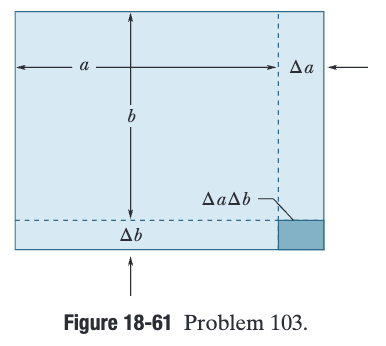
\includegraphics[width=0.25\textwidth]{picture_18-61.png} 
            % \label{fig:wrapfig}
        \end{wrapfigure}
        The area $A$ of a rectangular plate is $ab = 1.4 \unit{\meter^2}$. 
        Its coefficient of linear expansion is $\alpha = 32 \times 10^{-6} /\unit{\celsius}$. 
        After a temperature rise $\Delta T = 89\unit{\celsius}$, side $a$ is longer by $\Delta a$ and side $b$ is longer by $\Delta b$ (Fig. 18-61). 
        Neglecting the small quantity $(\Delta a \Delta b)/ab$, find $\Delta A$. 

        \subsection{Solution}
            We have a known equation of the change in length.
            \begin{equation}
                \Delta L    =   L \alpha \Delta T
            \end{equation}

            We can apply this to both $\Delta a$ and $\Delta b$.
            \begin{align}
                \Delta a    &=  a (32 \times 10^{-6} /\unit{\celsius}) (89 \unit{\celsius})\\
                \Delta b    &=  b (32 \times 10^{-6} /\unit{\celsius}) (89 \unit{\celsius})
            \end{align}

            Multiply $\Delta a$ by the width $b$ and $\Delta b$ by the height $a$. 
            We know following this the value of $ab$.
            \begin{align}
                b \Delta a  &=  ab (32 \times 10^{-6} /\unit{\celsius}) (89 \unit{\celsius})
                    =   (1.4 \unit{\meter^2}) (32 \times 10^{-6} /\unit{\celsius}) (89 \unit{\celsius})\\
                a \Delta b  &=  ab (32 \times 10^{-6} /\unit{\celsius}) (89 \unit{\celsius})
                    =   (1.4 \unit{\meter^2}) (32 \times 10^{-6} /\unit{\celsius}) (89 \unit{\celsius})
            \end{align}

            We can add these together to find $\Delta A$.
            \begin{align}
                \Delta A    &=  b \Delta a + a \Delta b
                    =   2 * (1.4 \unit{\meter^2}) (32 \times 10^{-6} /\unit{\celsius}) (89 \unit{\celsius})
                    =   \boxed{7.97 \times 10^{-3} \unit{\meter^2}}
            \end{align}
        
        \subsection{Remark on the $\Delta V$ Formula}
            It is notable that in this case, we can look at the equation out initial equation turned roughly into.
            \begin{gather}
                \Delta A    =   A (2\alpha) \Delta T
            \end{gather}

            We can recall from the textbook that the change in volume has a similar formula.
            \begin{gather}
                \Delta V    =   V (3\alpha) \Delta T
            \end{gather}

            This does beg the question of whether latter is ignoring some part of the volume, the same way we are considering $(\Delta a \Delta b)/ab$ negligible. 
            

    \pagebreak
    \section{Problem 105}
        A pendulum clock with a pendulum made of brass is designed to keep accurate time at 23°C. 
        Assume it is a simple pendulum consisting of a bob at one end of a brass rod of negligible mass that is pivoted about the other end. 
        If the clock operates at 0.0°C, (a) does it run too fast or too slow, and (b) what is the magnitude of its error in seconds per hour?

        \subsection{Solution (a)}
            There is no explanation of the operation of the clock relative to the pendulum.
            There are a small handful of values relevant to brass that could be of use.
            Brass has specific heat $c = 380 \unit{\frac{\joule}{\kilo\gram\cdot\kelvin}}$. 
            The material's thermal conductivity $k = 109 \unit{\watt/\meter\cdot\kelvin}$. 

            Suppose that the brass bob has mass $m$ and that its maximum height is $h$. 
            If the object has changed with its environment's temperature, it would thusly lower in its energy.
            \begin{align}
                Q   &=  cm (T_f - T_i)
            \end{align}

            Assuming all else to be equal, this would be the only change in energy.
            \begin{align}
                \Delta E    &=  Q
                    =   cm (T_f - T_i)
            \end{align}

            Since $\Delta T = T_f - T_i = -22 \unit{\kelvin}$ is negative, $c$ is positive, and $m$ cannot be negative (so far), $\Delta E$ must be negative.
            This means the maximum potential and kinetic energy of the clock is lower, and as such the maximum height and velocity are both lower.
            This means that the frequency of the bob will be greater.
            The clock will run \boxed{too\ fast}. 

        \subsection{Solution (b)}
            We should also note that the length of the pendulum will be shorter due to the temperature change. 
            The period of a simple pendulum is a simple formula.
            \begin{equation}
                T   =   2\pi f = 2\pi \sqrt{\frac{L}{g}}
            \end{equation}

            The only changing value is $L$.
            We can include this in the ratio between the time to the change in time.
            We can also take the derivative of $L$ to get $dL$ and its formula.
            \begin{gather}
                L(T)    =   L_0 (1 + \alpha T(t))\\
                \dv{L}{T}   =   L_0 \alpha\\
                \dv{L}{T} \cdot \Delta T    =   L_0 \alpha \Delta T \approx dL
            \end{gather}

            This can in turn be used for the fraction involving $\Delta T$ we are looking for.
            \begin{gather}
                T   =   2\pi \sqrt{\frac{L}{g}}\\
                \dv{T}{L}   =   \pi \frac{1}{\sqrt{gL}}\\
                dT  =   \pi \frac{1}{\sqrt{gL}}\,dL \approx \Delta T\\
                \begin{align}
                    \frac{\Delta T}{T}  &\approx    \frac{dT}{T}
                        =   \frac{\pi \frac{1}{\sqrt{gL}}}{2\pi \sqrt{\frac{L}{g}}}\,dL
                        =   \frac{1}{2L}\,dL
                \end{align}
            \end{gather}

            We can operate on this.
            \begin{align}
                \frac{\Delta T}{T}  &\approx    \frac{1}{2L}\,dL
                    \approx \frac{L_0 \alpha \Delta T}{2L}
                    \approx \frac{1}{2} \alpha \Delta T\\
                    &\approx    \frac{1}{2} (19 \times 10^{-6}) (23)
                    =   2.185 \times 10^{-4} * 3600 \unit{\second/\hour}\\
                    &=  \boxed{0.7866 \unit{\second/\hour}}
            \end{align}

    \pagebreak

    \tableofcontents
\end{document}